\documentclass[tikz]{article}
\usepackage{graphicx}
\usepackage{tikz}
\usepackage{float}
\usetikzlibrary{arrows,decorations.markings}

\begin{document}
\begin{figure}[H]
	\begin{center}
		\begin{tikzpicture}[scale=0.9]
		\begin{scope}[decoration={markings,mark=at position 0.6 with {\arrow[scale=2,>=stealth]{>}}}]
		% Draw vertex line
		\draw (0,0) [dashed] -- (1,0);
		
		% Draw incoming line
		\draw [postaction={decorate}] (-0.5,1) -- (0,0);
		
		% Draw outgoing line
		\draw [postaction={decorate}] (0,0) -- (-0.5,-1);
		
		% Draw vertex point
		\filldraw (1,0) circle (0.05cm);
		\end{scope}
		
		\begin{scope}[xshift=4cm, decoration={markings,mark=at position 0.6 with {\arrow[scale=2,>=stealth]{>}}}]
		% Draw vertex line
		\draw (0,0) [dashed] -- (1,0);
		
		% Draw outgoing line
		\draw [postaction={decorate}] (0,0) -- (-0.5,1);
		
		% Draw incoming line
		\draw [postaction={decorate}] (-0.5,-1) -- (0,0);
		
		% Draw vertex point
		\filldraw (1,0) circle (0.05cm);
		\end{scope}
		
		\begin{scope}[xshift=8cm, decoration={markings,mark=at position 0.6 with {\arrow[scale=2,>=stealth]{>}}}]
		% Draw vertex line
		\draw (0,0) [dashed] -- (1,0);
		
		% Draw outgoing line
		\draw [postaction={decorate}] (0,0) -- (0.5,-1);
		
		% Draw incoming line
		\draw [postaction={decorate}] (-0.5,-1) -- (0,0);
		
		% Draw vertex point
		\filldraw (1,0) circle (0.05cm);
		\end{scope}
		
		\begin{scope}[xshift=12cm, decoration={markings,mark=at position 0.6 with {\arrow[scale=2,>=stealth]{>}}}]
		% Draw vertex line
		\draw (0,0) [dashed] -- (1,0);
		
		% Draw outgoing line
		\draw [postaction={decorate}] (0,0) -- (-0.5,1);
		
		% Draw incoming line
		\draw [postaction={decorate}] (0.5,1) -- (0,0);
		
		% Draw vertex point
		\filldraw (1,0) circle (0.05cm);
		\end{scope}
		\end{tikzpicture}
	\end{center}
	%\caption{Ground state of Helium.}
	\label{fig:three}
\end{figure}


\newpage
\begin{figure}[H]
	\begin{center}
		\begin{tikzpicture}[scale=2.5]
		\begin{scope}[decoration={markings,mark=at position 0.6 with {\arrow[scale=2,>=stealth]{>}}}]
		
		% Hamiltonian
		% Draw vertex line
		\draw (0,0) [dashed] -- (1.5,0);
		
		% Draw incoming lines
		\draw [postaction={decorate}] (0.5,-1) -- (0,0);
		\draw [postaction={decorate}] (2,-1) -- (1.5,0);
		
		% Draw outgoing lines
		\draw [postaction={decorate}] (0,0) -- (-0.5,-1);
		\draw [postaction={decorate}] (1.5,0) -- (1,-1);
		
		
		% Draw connection lines
		\draw (0.5,-1) [dotted] -- (1,-2);
		\draw (1,-1) [dotted] -- (0.5,-2);
		\draw (-0.5,-1) [dotted] -- (-1,-2);
		\draw (2,-1) [dotted] -- (2.5,-2);
		
		
		% Left T2
		% Draw vertex line
		\draw (0,-3) [dashed] -- (-1.5,-3);
		
		% Draw incoming lines
		\draw [postaction={decorate}] (-1,-2) -- (-1.5,-3);
		\draw [postaction={decorate}] (0.5,-2) -- (0,-3);
		
		% Draw outgoing lines
		\draw [postaction={decorate}] (-1.5,-3) -- (-2,-2) node[midway, left] (a){a};
		\draw [postaction={decorate}] (0,-3) -- (-0.5,-2) node[midway, left] (b){b};
		
		
		% Right T2
		% Draw vertex line
		\draw (3,-3) [dashed] -- (1.5,-3);
		
		% Draw incoming lines
		\draw [postaction={decorate}] (2,-2) -- (1.5,-3) node[midway, right] (i){i};
		\draw [postaction={decorate}] (3.5,-2) -- (3,-3) node[midway, right] (j){j};
		
		% Draw outgoing lines
		\draw [postaction={decorate}] (1.5,-3) -- (1,-2);
		\draw [postaction={decorate}] (3,-3) -- (2.5,-2);
		
		
		% Draw vertex point
		%\filldraw (1,0) circle (0.05cm);
		\end{scope}
		
		\end{tikzpicture}
	\end{center}
	%\caption{Ground state of Helium.}
	\label{fig:four}
\end{figure}

\newpage

\begin{figure}[H]
	\begin{center}
		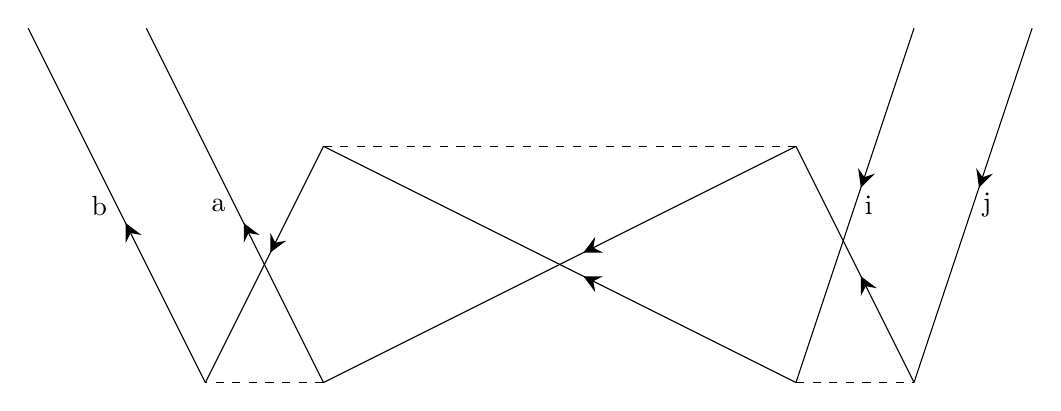
\begin{tikzpicture}[scale=3]
		\begin{scope}[decoration={markings,mark=at position 0.45 with {\arrow[scale=2,>=stealth]{>}}}]
		
		% Hamiltonian
		% Draw vertex line
		\draw (0,0) [dashed] -- (2,0);
		
		% Draw incoming lines
		\draw [postaction={decorate}] (0,0) -- (-0.5,-1);
		\draw [postaction={decorate}] (2,0) -- (0,-1);
		
		% Draw outgoing lines
		\draw [postaction={decorate}] (2,-1) -- (0,0);
		\draw [postaction={decorate}] (2.5,-1) -- (2,0);
		
		
		% Left T2
		% Draw vertex line
		\draw (0,-1) [dashed] -- (-0.5,-1);
		
		% Draw outgoing lines
		\draw [postaction={decorate}] (0,-1) -- (-0.75,0.5) node[midway, left] (a){a};
		\draw [postaction={decorate}] (-0.5,-1) -- (-1.25,0.5) node[midway, left] (b){b};
		
		
		% Right T2
		% Draw vertex line
		\draw (2,-1) [dashed] -- (2.5,-1);
		
		% Draw incoming lines
		\draw [postaction={decorate}] (2.5,0.5) -- (2,-1) node[midway, right] (i){i};
		\draw [postaction={decorate}] (3,0.5) -- (2.5,-1) node[midway, right] (j){j};
		
		
		% Draw vertex point
		%\filldraw (1,0) circle (0.05cm);
		\end{scope}
		
		\end{tikzpicture}
	\end{center}
	%\caption{Ground state of Helium.}
	\label{fig:five}
\end{figure}

\end{document}